\documentclass[conference]{IEEEtran}

\usepackage{amsmath,amssymb,amsfonts}
\usepackage{algorithmic}
\usepackage{graphicx}
\usepackage{textcomp}
\usepackage{xcolor}
\def\BibTeX{{\rm B\kern-.05em{\sc i\kern-.025em b}\kern-.08em
    T\kern-.1667em\lower.7ex\hbox{E}\kern-.125emX}}

% setup BibTex
\usepackage[
backend=biber,
style=ieee,
url=false,
isbn=false,
eprint=false
]{biblatex}
\addbibresource{references.bib}

% utility 
\usepackage{microtype}
\usepackage{siunitx}
%\usepackage[capitalise]{cleverref}
\begin{document}


\title{Effects of Compressive Stress on Ferrites in Inductive Power Transfer}

\author{
  Alexander K. Bailey, Jerry Sun\textsuperscript{\textdagger}, Seho Kim, Willsen Wijaya\textsuperscript{\textdagger}, Tom Allen\textsuperscript{\textdagger}, Grant A. Covic\\
  \textit{Department of Electrical, Computer and Software Engineering}\\
  \textit{\textsuperscript{\textdagger}Centre for Advanced Materials Manufacturing and Design}\\
  \textit{University of Auckland}\\
  Auckland, New Zealand\\
  \{alexander.bailey, jerry.sun, seho.kim, willsen.wijaya, tom.allen, ga.covic\}@auckland.ac.nz\\ 
}
\maketitle

\begin{abstract}
  Inductive power transfer (IPT) magnetics are often `potted' with an encapsulant material to improve thermal performance.
  The difference in thermal expansion between common epoxy based encapsulant materials and ceramic ferrites creates a compressive load which permanently reduces the magnetic performance of the core material. 
  This article measures how the core loss of Mn--Zn ferrites changes with an applied compressive stress of \SIrange{10}{100}{\mega\pascal} at \SI{85}{\kilo\hertz}. 
  The measured data is used to predict how core losses change in a practical potted IPT pad, demonstrating a \SI{140}{\percent} increase in core loss. 
\end{abstract}

\begin{IEEEkeywords}
Core loss, inductive power transfer (IPT), loss measurement, magnetic losses
\end{IEEEkeywords}

\section{Introduction}

\IEEEPARstart{E}{lectric} vehicles (EVs) are increasingly common due to lowering costs and a rising need for climate change. 
However, existing infrastructure favours the outgoing Internal Combustion Engine Vehicles (ICEVs), meaning charging EVs can be cumbersome. 
Inductive power transfer (IPT) is a wireless charging technology that enables power transfer using magnetic fields. 
The application of this technology to the charging of EVs could enable more reliable and convenient charging of EVs of all power levels \cite{covicModernTrendsInductive2013b}. 

At higher power levels, thermal issues limit power density. 
In order to improve the thermal performance of the IPT magnetics, both the coil and core layer (shown in \ref{fig:padstructure}) are `potted' in an encapsulant material \cite{kneidlProcessingInfluencesResinbased2020}. 
Typical encapsulant materials are resin-based with high toughness and thermal conductivity which improves the temperature profile uniformity and allows for a higher current density in the coil. 
However, several articles have noted the deterimental effect of encapsulant materials on the magnetic performance of ferrites. 

Polycrystalline ferrites show decreased magnetic permeability and a widening $B$-$H$ curve under applied pressure due to the compressed topography of the domain walls \cite{leflochEffectPressureSoft1981}. 
Foote et. al verified the reduction in permeability and increased core loss through the construction of a small-scale potted IPT coil assembly, demonstrating a \SI{\sim 100}{\percent} increase in losses \cite{footeEncapsulationResidualStress2023}.
This article aims to measure the effect of pressure on ferrite core loss at \SI{85}{\kilo\hertz} in a material independent and reproducable manner such that designers can better predict the impacts of encapsulation on the IPT system's behaviour. 

\begin{figure}[t]
  \centering
  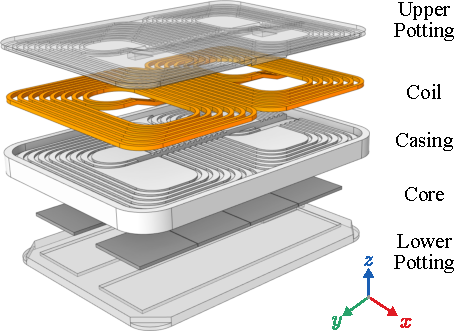
\includegraphics{figures/padstructure.pdf}
  \caption{Typical structure of IPT pad for EV charging}
  \label{fig:padstructure}
\end{figure}

\section{Characterisation of Ferrite Under Stress}

The core loss $P_\text{core}$ is measured using a partial cancellation method which modifies the conventional two-winding method with a compensation capacitor $C_s$ in series to cancel the reactive voltage across the inductor under test $L_t$ \cite{houNewHighFrequencyCore2017}. 
The equivalent circuit of this method is shown in \ref{fig:partialcancellationcircuit}.
$C_s$ could be selected to completely cancel the reactive power in the system, but maintaining resonance for different operating conditions is challenging. 
Instead, a partial cancellation method defines a voltage cancellation factor $k_v$, the ratio of the cancelled reactive voltage to the total reactive voltage, to only `partially' cancel the reactive component of $L_t$. 
The core loss can then be found from measurements of the current flowing through the primary winding $i_L(t)$, the voltage on the secondary winding $v_2(t)$ and the voltage across the compensation capacitor $v_C(t)$. 
\begin{equation}
  P_\text{core} = f \int_0^T v_2(t)i_L(t)dt + \frac{f}{k_v} \int_0^T v_c(t)i_L(t) dt
\end{equation}
\begin{equation}
  P_\text{core}^{\prime} = f \int_0^T v_2(t)i_L^{\prime} (t)dt + \frac{f}{k_v} \int_0^T v_c(t)i_L^{\prime}(t) dt
\end{equation}
\begin{equation}
  k_v = \frac{\int_0^T v_c(t)i_L(t)dt - \int_0^T v_ci_L^\prime(t)dt}{\int_0^T v_2(t) i_L^\prime(t) dt - \int_0^T v_2(t) i_L(t) dt}
\end{equation}

\begin{figure}[t]
  \centering
  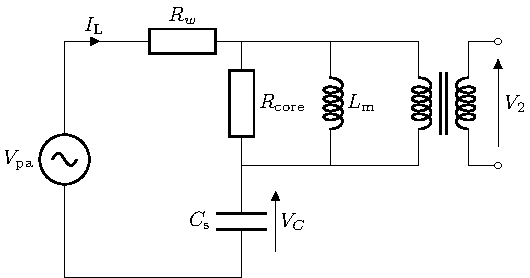
\includegraphics[width=3.5in, height=2in]{partialcancellationcircuit.pdf}
  \caption{Equivalent circuit of the partial cancellation method}
  \label{fig:partialcancellationcircuit}
\end{figure}

\section{Verification of Core Loss Measurements}

\section{Conclusion}

\section*{References}
\printbibliography[heading=none]


\end{document}
